\documentclass[11pt]{article}

\usepackage{geometry}
\usepackage[scaled]{berasans}
\renewcommand*\familydefault{\sfdefault}  
\usepackage[T1]{fontenc}
\usepackage[dvipsnames]{xcolor}             % font packages
\renewcommand{\baselinestretch}{1.5}        % line spacing
\usepackage{parskip}                        % paragraph spacing
\usepackage{listings}                       % for listings of the code
\usepackage{graphicx}                       % for images
\usepackage{array}                          % for tables
\usepackage{hyperref}
\usepackage{graphicx}
\usepackage{caption}

\lstdefinestyle{mystyle}{
    backgroundcolor=\color{white},   
    commentstyle=\color{PineGreen},
    keywordstyle=\color{BrickRed},
    numberstyle=\tiny\color{gray},
    stringstyle=\color{Mulberry},
    basicstyle=\ttfamily\footnotesize,
    breakatwhitespace=false,         
    breaklines=true, 
    captionpos=b,                    
    keepspaces=true,                 
    numbers=left,                    
    numbersep=5pt,                  
    showspaces=false,                
    showstringspaces=false,
    showtabs=false,                  
    tabsize=2
}
\lstset{style=mystyle}

\title{
    \scshape\Huge\textbf{Football Network}
    \\\Huge\textbf{Management System} 
    \\\Large Database Programming
    \\\large\textit {Project Report} 
    \\\vspace{2em}
}
\author{
    Tycjan Fortuna \\\textit{Team leader}\\ID: 242213
        \and
    Filip Krylecki\\ID: 242220
        \and
    Marek Kopania\\ID: 234760
        \and
    Paulina Klewin\\ID: 247028
        \vspace{3em}
    \\Information Technology\\IFE, 4th semester\\Compulsory course
        \vspace{2em}
}
\date{May 29, 2023}

\begin{document}
\maketitle \thispagestyle{empty} \clearpage

\small \tableofcontents
\clearpage

\small \lstlistoflistings
\clearpage

\section{Project description}
\subsection{Problem description}
Our client wants a management system to keep information about the professional football division of the Spanish football league system, La Liga. They wish to keep and update relevant information, i.e. about the matches, participating football clubs, stadiums and varied tickets. Throughout the season, twenty football teams compete against each other twice, at home and away, resulting in 38 matches per club. The client wants to know which three teams are the best in La Liga. They can display record of currently playing football players as well as detailed information on each individual. The client can search for teams and stadiums by given city. Additionally, it is possible for them to generate a report containing scores of the matches registered in the database. Thanks to our management system the client can see the average remuneration of football players from a selected club. There is a possibility to check how commercially successful any of the matches was. Employees of our client are able to maintain the information about La Liga's progress by adding new data and updating the existing one. They can also parse XML report. Our client requested verification of the data that is entered into the system.

\subsection{Aims}
The aim of the management system is to maintain the information for the client's purposes, including its storage and display. The management system enables maintenance of large amounts of data, allowing further expansion with data from following seasons of La Liga. The system must fulfill the requests of the client as well as verify correctness of the input data. The up-to-date information is displayed in a manner requested by the client.

\subsection{System features and functions}
The football network management system allows:
\begin{itemize}
    \item alteration and storage of data concerning matches
    \item alteration and storage of data concerning football teams and their members
    \item alteration and storage of data concerning stadiums
    \item alteration and storage of data concerning tickets sold for the matches
    \item verification of input data
\end{itemize}

\subsection{Entity Relationship Diagram (ERD)}
\vspace{2em}
\begin{figure}[htp]
    \centering
    \rotatebox{90}{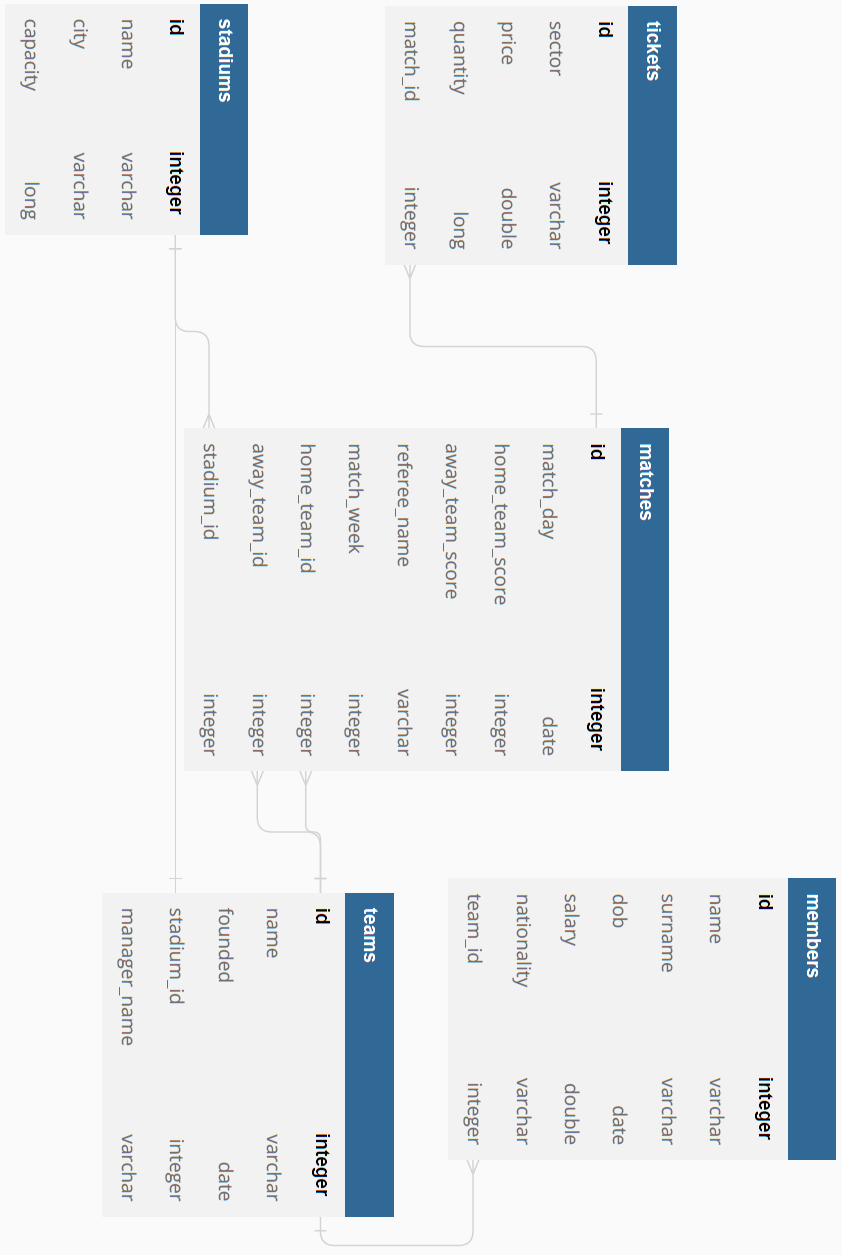
\includegraphics[height=\linewidth]{Images/erd15.png}}
    \label{fig:ERD}
\end{figure}

\clearpage

\section{Implementation}
\subsection{Scripts for creating the database}
\begin{lstlisting}[language=SQL, caption=\small Scripts creating the database (\texttt{DBTableCreation.sql} file)]
-- Create Stadiums table
CREATE TABLE stadiums (
  id NUMBER GENERATED BY DEFAULT ON NULL AS IDENTITY,
  name VARCHAR2(255),
  city VARCHAR2(255),
  capacity NUMBER,
  PRIMARY KEY (id)
);

-- Create Teams table
CREATE TABLE teams (
  id NUMBER GENERATED BY DEFAULT ON NULL AS IDENTITY,
  name VARCHAR2(255),
  founded DATE,
  stadium_id NUMBER,
  manager_name VARCHAR2(255),
  PRIMARY KEY (id),
  FOREIGN KEY (stadium_id) REFERENCES stadiums(id)
);

-- Create Matches table
CREATE TABLE matches (
  id NUMBER GENERATED BY DEFAULT ON NULL AS IDENTITY,
  match_date DATE,
  home_team_score NUMBER,
  away_team_score NUMBER,
  referee_name VARCHAR2(255),
  match_week NUMBER,
  home_team_id NUMBER,
  away_team_id NUMBER,
  stadium_id NUMBER,
  PRIMARY KEY (id),
  FOREIGN KEY (stadium_id) REFERENCES stadiums(id),
  FOREIGN KEY (home_team_id) REFERENCES teams(id),
  FOREIGN KEY (away_team_id) REFERENCES teams(id)
);

-- Create Tickets table
CREATE TABLE tickets (
  id NUMBER GENERATED BY DEFAULT ON NULL AS IDENTITY,
  sector VARCHAR2(255),
  price NUMBER,
  quantity NUMBER,
  match_id NUMBER,
  PRIMARY KEY (id),
  FOREIGN KEY (match_id) REFERENCES matches(id)
);

-- Create Members table
CREATE TABLE members (
  id NUMBER GENERATED BY DEFAULT ON NULL AS IDENTITY,
  name VARCHAR2(255),
  surname VARCHAR2(255),
  dob DATE,
  salary NUMBER,
  nationality VARCHAR2(255),
  team_id NUMBER,
  PRIMARY KEY (id),
  FOREIGN KEY (team_id) REFERENCES teams(id)
);
\end{lstlisting}
\subsection{Scripts for populating the database}
\begin{lstlisting}[language=SQL, caption=\small Scripts populating the database (\texttt{DBTableInsertion.sql} file)]
-- Populate Stadiums table
INSERT INTO stadiums VALUES (1,'Camp Nou','Barcelona',99354);
INSERT INTO stadiums VALUES (2,'Estadio Metropolitano','Madrid',68456);
(...)
INSERT INTO stadiums VALUES (9,'Campo de Futbol de Vallecas','Puente de Vallecas',14708);
INSERT INTO stadiums VALUES (10,'El Sadar','Pamplona',23576);

-- Populate Teams table
INSERT INTO teams VALUES (1,'Barcelona',TO_DATE('1899-11-29', 'YYYY-MM-DD'),1,'Xavier Hernandez Creus');
INSERT INTO teams VALUES (2,'Atletico Madrid',TO_DATE('1903-04-26', 'YYYY-MM-DD'),2,'Diego Simeone');
(...)
INSERT INTO teams VALUES (9,'Rayo Vallecano de Madrid',TO_DATE('1919-03-18', 'YYYY-MM-DD'),9,'Andoni Iraola');
INSERT INTO teams VALUES (10,'Osasuna',TO_DATE('1890-01-25', 'YYYY-MM-DD'),10,'Jagoba Arrasate');

-- Populate Matches table
INSERT INTO matches VALUES (1, TO_DATE('2023-08-05', 'YYYY-MM-DD'), 3, 2, 'Antonio Mateu Lahoz', 1, 1, 2, 1);
INSERT INTO matches VALUES (2, TO_DATE('2023-08-05', 'YYYY-MM-DD'), 1, 0, 'Carlos Del Cerro Grande', 1, 3, 4, 3);
(...)
INSERT INTO matches VALUES (249, TO_DATE('2025-04-20', 'YYYY-MM-DD'), 1, 0, 'Carlos Del Cerro Grande', 3, 6, 1, 6);
INSERT INTO matches VALUES (250, TO_DATE('2025-04-26', 'YYYY-MM-DD'), 1, 1, 'Aliyar Aghayev', 4, 7, 10, 7);

-- Populate Tickets table
INSERT INTO tickets VALUES (1, 'A', 50.00, 10000, 1);
INSERT INTO tickets VALUES (2, 'B', 40.00, 15000, 1);
(...)
INSERT INTO tickets VALUES (979, 'B', 1255.00, 9670, 250);
INSERT INTO tickets VALUES (980, 'A', 1245.00, 9680, 250);

-- Populate Members table
INSERT INTO members VALUES (1,'Marc-Andre','ter Stegen',TO_DATE('1992-04-30', 'YYYY-MM-DD'),8900.99,'German',1);
INSERT INTO members VALUES (2,'Ronald','Araujo',TO_DATE('1999-03-07', 'YYYY-MM-DD'),7858.09,'Uruguayan',1);
(...)
INSERT INTO members VALUES (107,'Lucas','Torro',TO_DATE('1994-01-01', 'YYYY-MM-DD'),9876.00,'Spanish',10);
INSERT INTO members VALUES (108,'Jony','Rodriguez',TO_DATE('1991-01-01', 'YYYY-MM-DD'),9876.00,'Spanish',10);
\end{lstlisting}
\vspace{2em}
\subsection{SQL queries}
\begin{lstlisting}[language=SQL, caption=\small SQL queries (\texttt{DBQueries.sql} file), escapeinside={(*@}{@*)}]
-- Basic queries for our database
SELECT * FROM stadiums;

SELECT * FROM teams;

SELECT * FROM matches;

SELECT * FROM tickets;

SELECT * FROM members;

-- 1) Retrieve the stadium details for a specific team:
SELECT stadiums.* FROM stadiums
    JOIN teams ON stadiums.id = teams.stadium_id
WHERE teams.name = 'Barcelona';
(*@
\begin{figure}[htp]
    \centering
    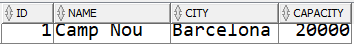
\includegraphics[width=6cm]{Images/query1.png}
    \caption{\small \texttt{Query 1} output}
    \label{fig:query1}
\end{figure}
@*)    

-- 2) Retrieve the matches played in a specific stadium:
SELECT * FROM matches
WHERE stadium_id = 1;
(*@
\begin{figure}[htp]
    \centering
    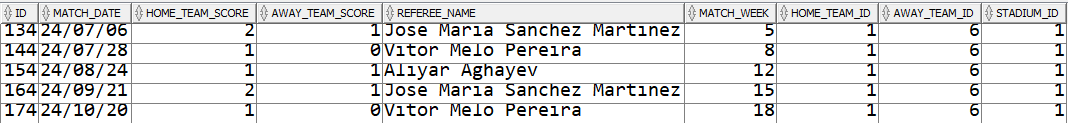
\includegraphics[width=15cm]{Images/query2.png}
    \caption{\small \texttt{Query 2} output}
    \label{fig:query2}
\end{figure}
@*)

-- 3) Retrieve the teams playing in a specific match:
SELECT home_teams.name AS home_team,
       away_teams.name AS away_team
FROM matches
    JOIN teams home_teams ON home_teams.id = matches.home_team_id
    JOIN teams away_teams ON away_teams.id = matches.away_team_id
WHERE matches.id = 11;
(*@
\begin{figure}[htp]
    \centering
    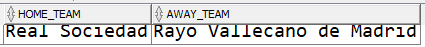
\includegraphics[width=8cm]{Images/query3.png}
    \caption{\small \texttt{Query 3} output}
    \label{fig:query3}
\end{figure}
\clearpage
@*)
-- 4) Retrieve all tickets for a specific match:
SELECT * FROM tickets
WHERE match_id = 1;
(*@
\begin{figure}[htp]
    \centering
    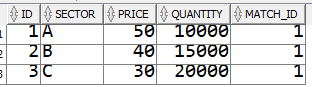
\includegraphics[width=5cm]{Images/query4.png}
    \caption{\small \texttt{Query 4} output}
    \label{fig:query4}
\end{figure}
@*)

-- 5) Retrieve the members of a specific team:
SELECT * FROM members
WHERE team_id = 5;
(*@
\begin{figure}[htp]
    \centering
    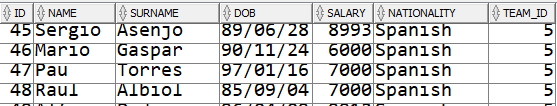
\includegraphics[width=10cm]{Images/query5.png}
    \caption{\small \texttt{Query 5} output}
    \label{fig:query5}
\end{figure}
@*)

-- 6) Retrieve the average ticket price for each match:
SELECT matches.id,
       AVG(tickets.price) AS average_ticket_price
FROM matches
    JOIN tickets ON matches.id = tickets.match_id
GROUP BY matches.id;
(*@
\clearpage
\begin{figure}[htp]
    \centering
    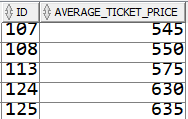
\includegraphics[width=3cm]{Images/query6.png}
    \caption{\small \texttt{Query 6} output}
    \label{fig:query6}
\end{figure}
@*)

-- 7) Retrieve the team with the highest average score in home matches:
SELECT teams.name,
       AVG(matches.home_team_score) AS average_home_score
FROM teams
    JOIN matches ON teams.id = matches.home_team_id
GROUP BY teams.name
ORDER BY average_home_score DESC
FETCH FIRST ROW ONLY;
(*@
\begin{figure}[htp]
    \centering
    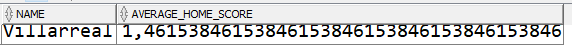
\includegraphics[width=10cm]{Images/query7.png}
    \caption{\small \texttt{Query 7} output}
    \label{fig:query7}
\end{figure}
@*)

-- 8) Retrieve the matches where the home team scored more than the away team:
SELECT matches.* FROM matches
WHERE home_team_score > away_team_score;
(*@
\begin{figure}[htp]
    \centering
    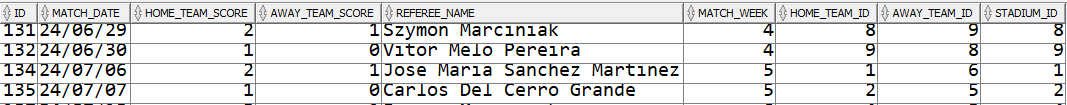
\includegraphics[width=15cm]{Images/query8.png}
    \caption{\small \texttt{Query 8} output}
    \label{fig:query8}
\end{figure}
\clearpage
@*)
-- 9) Retrieve the top 5 stadiums with the highest average of score 
SELECT stadiums.name,
       AVG(matches.home_team_score + matches.away_team_score) AS average_score
FROM stadiums
    JOIN matches ON stadiums.id = matches.stadium_id
GROUP BY stadiums.name
ORDER BY average_score DESC
FETCH FIRST 5 ROWS ONLY;
(*@
\begin{figure}[htp]
    \centering
    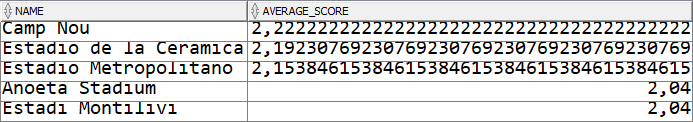
\includegraphics[width=12cm]{Images/query9.png}
    \caption{\small \texttt{Query 9} output}
    \label{fig:query9}
\end{figure}
@*)

-- 10) Retrieve the matches where the ticket quantity sold is greater than the average ticket quantity sold for all matches:
SELECT matches.* FROM matches
    JOIN tickets ON matches.id = tickets.match_id
WHERE tickets.quantity > (SELECT AVG(quantity) FROM tickets);
(*@
\begin{figure}[htp]
    \centering
    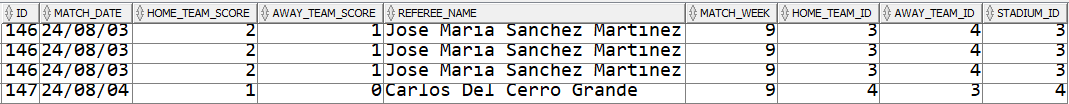
\includegraphics[width=15cm]{Images/query10.png}
    \caption{\small \texttt{Query 10} output}
    \label{fig:query10}
\end{figure}
@*)

-- 11) Retrieve the teams with the highest number of members:
SELECT teams.name,
       COUNT(members.id) AS members_count
FROM teams
    JOIN members ON teams.id = members.team_id
GROUP BY teams.name
ORDER BY members_count DESC;
(*@
\begin{figure}[htp]
    \centering
    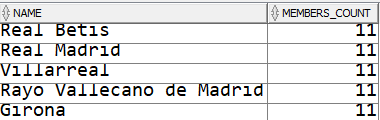
\includegraphics[width=7cm]{Images/query11.png}
    \caption{\small \texttt{Query 11} output}
    \label{fig:query11}
\end{figure}
@*)

-- 12) Retrieve the team with the highest average member salary:
SELECT teams.name,
       AVG(members.salary) AS average_salary
FROM teams
    JOIN members ON teams.id = members.team_id
GROUP BY teams.name
ORDER BY average_salary DESC
FETCH FIRST ROW ONLY;
(*@
\begin{figure}[htp]
    \centering
    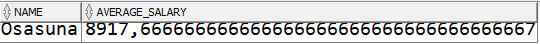
\includegraphics[width=10cm]{Images/query12.png}
    \caption{\small \texttt{Query 12} output}
    \label{fig:query12}
\end{figure}
@*)

-- 13) Retrieve the matches where both home and away teams scored more than the average score in all matches:
SELECT matches.* FROM matches
WHERE home_team_score > (SELECT AVG(home_team_score) FROM matches)
    AND away_team_score > (SELECT AVG(away_team_score) FROM matches);
(*@
\clearpage
\begin{figure}[htp]
    \centering
    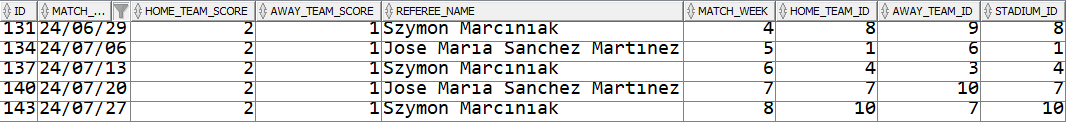
\includegraphics[width=15cm]{Images/query13.png}
    \caption{\small \texttt{Query 13} output}
    \label{fig:query13}
\end{figure}
@*)

-- 14) Retrieve the members who have a salary higher than the average salary of all members:
SELECT * FROM members
WHERE salary > (SELECT AVG(salary) FROM members);
(*@
\begin{figure}[htp]
    \centering
    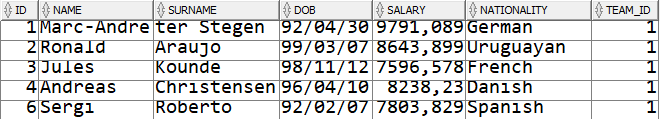
\includegraphics[width=13cm]{Images/query14.png}
    \caption{\small \texttt{Query 14} output}
    \label{fig:query14}
\end{figure}
@*)

-- 15) Retrieve the stadiums that have hosted matches with a match week greater than 10:
SELECT UNIQUE stadiums.* FROM stadiums
    JOIN matches ON stadiums.id = matches.stadium_id
WHERE matches.match_week > 10;
(*@
\begin{figure}[htp]
    \centering
    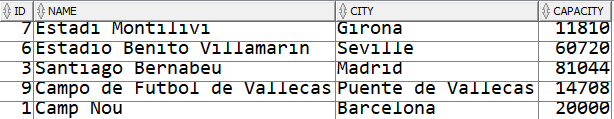
\includegraphics[width=12cm]{Images/query15.png}
    \caption{\small \texttt{Query 15} output}
    \label{fig:query15}
\end{figure}
\clearpage
@*)
-- 16) Retrieve the teams and their total ticket sales (quantity * price) for a specific match:
SELECT teams.name                            AS team_name,
       SUM(tickets.quantity * tickets.price) AS total_sales
FROM teams
    JOIN matches ON teams.id = matches.home_team_id
                    OR teams.id = matches.away_team_id
    JOIN tickets ON matches.id = tickets.match_id
WHERE matches.id = 2
GROUP BY teams.name;
(*@
\begin{figure}[htp]
    \centering
    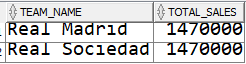
\includegraphics[width=5cm]{Images/query16.png}
    \caption{\small \texttt{Query 16} output}
    \label{fig:query16}
\end{figure}
@*)
\end{lstlisting}
\vspace{2em}
\subsection{Procedures}
\begin{lstlisting}[language=SQL, caption=\small Procedures (\texttt{DBProcedures.sql} file), escapeinside={(*@}{@*)}]
-- Update salary of players of given football club by certain percentage
CREATE OR REPLACE PROCEDURE update_salary (
    p_team_id             NUMBER,
    p_percentage_increase NUMBER
) IS
    CURSOR member_cur IS
    SELECT id,
           salary
    FROM members
    WHERE team_id = p_team_id;

    v_member_id  NUMBER;
    v_new_salary NUMBER;
BEGIN
    OPEN member_cur;
    
    LOOP
        FETCH member_cur INTO v_member_id,
                              v_new_salary;
        EXIT WHEN member_cur%notfound;
        
        v_new_salary := v_new_salary + ( v_new_salary * p_percentage_increase / 100 );
        
        UPDATE members
        SET salary = v_new_salary
        WHERE id = v_member_id;
    END LOOP;

    CLOSE member_cur;
    COMMIT;
EXCEPTION
    WHEN OTHERS THEN
        dbms_output.put_line('Error while increasing salary!');
END;

-- Example of update_salary usage
-- BEGIN
--     update_salary(1, 10);
-- END;


-- Retrieving data about the football players
CREATE OR REPLACE PROCEDURE display_member_team IS
    v_name    members.name%TYPE;
    v_surname members.surname%TYPE;
    v_team    teams.name%TYPE;
    CURSOR member_cursor IS
    SELECT m.name,
           m.surname,
           t.name
    FROM members m
        LEFT JOIN teams   t ON m.team_id = t.id;

BEGIN
    OPEN member_cursor;
    
    LOOP
        FETCH member_cursor INTO v_name,
                                 v_surname,
                                 v_team;
        EXIT WHEN member_cursor%notfound;
        dbms_output.put_line(v_name
                             || ' '
                             || v_surname
                             || ' plays for '
                             || v_team);
    END LOOP;

    CLOSE member_cursor;
END;

-- Example of display_member_team usage
-- BEGIN
--     display_member_team;
-- END;
(*@
\clearpage
\begin{figure}[htp]
    \centering
    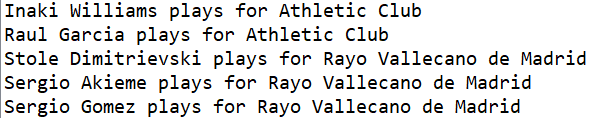
\includegraphics[width=10cm]{Images/procedure2.png}
    \caption{\small Procedure \texttt{display\_member\_team} output}
    \label{fig:procedure2}
\end{figure}
@*)


-- Retrieve data about which teams and stadiums are in a specific city
CREATE OR REPLACE PROCEDURE get_teams_and_stadiums_by_city (
    p_city VARCHAR2
) IS
    v_team_name    VARCHAR2(255);
    v_stadium_name VARCHAR2(255);
BEGIN
    SELECT t.name,
           s.name
    INTO v_team_name,
         v_stadium_name
    FROM teams t
        JOIN stadiums s ON t.stadium_id = s.id
    WHERE s.city = p_city;

    dbms_output.put_line('Team: '
                         || v_team_name
                         || ', Stadium: '
                         || v_stadium_name);
EXCEPTION
    WHEN no_data_found THEN
        dbms_output.put_line('No teams found for the specified city.');
    WHEN OTHERS THEN
        dbms_output.put_line('Error while fetching data: ' || sqlerrm);
END;(*@\clearpage@*)
-- Example of get_teams_and_stadiums_by_city usage
-- DECLARE
--     v_team_name    VARCHAR2(255);
--     v_stadium_name VARCHAR2(255);
-- BEGIN
--     get_teams_and_stadiums_by_city('Pamplona');
-- END;
(*@
\begin{figure}[htp]
    \centering
    
\includegraphics[width=7cm]{Images/procedure3.png}
    \caption{\small Procedure \texttt{get\_teams\_and\_stadiums\_by\_city} output}
    \label{fig:procedure3}
\end{figure}
@*)
\end{lstlisting}
\vspace{2em}
\subsection{Functions}
\begin{lstlisting}[language=SQL, caption=\small Functions (\texttt{DBFunctions.sql} file), escapeinside={(*@}{@*)}]
-- Calculate average salary of a specific football club
CREATE OR REPLACE FUNCTION calculate_average_salary_by_team (
    p_team_id NUMBER
) RETURN NUMBER AS
    v_total_salary   NUMBER := 0;
    v_member_count   NUMBER := 0;
    v_average_salary NUMBER := 0;
    no_members_exception EXCEPTION;
BEGIN
    FOR member_rec IN (SELECT salary
                       FROM members
                       WHERE team_id = p_team_id
    ) LOOP
        v_total_salary := v_total_salary + member_rec.salary;
        v_member_count := v_member_count + 1;
    END LOOP;

    IF v_member_count > 0 THEN
        v_average_salary := v_total_salary / v_member_count;
    ELSE
        RAISE no_members_exception;
    END IF;

    RETURN v_average_salary;
EXCEPTION
    WHEN no_members_exception THEN
        dbms_output.put_line('Error: ' || sqlerrm);
        RETURN NULL;
END;
/

-- Example of calculate_average_salary_by_team usage
-- DECLARE
--     v_avg_salary NUMBER;
-- BEGIN
--     v_avg_salary := calculate_average_salary_by_team(1);
--     dbms_output.put_line('Average Salary: ' || v_avg_salary);
-- END;
(*@
\begin{figure}[htp]
    \centering
    
\includegraphics[width=5cm]{Images/function1.png}
    \caption{\small Function \texttt{calculate\_average\_salary\_by\_team} output}
    \label{fig:function1}
\end{figure}
@*)


-- Calculate total revenue of a specific match
CREATE OR REPLACE FUNCTION calculate_total_revenue (
    p_match_id NUMBER
) RETURN NUMBER AS
    v_total_revenue NUMBER := 0;
    v_total_salary  NUMBER := 0;
    v_net_revenue   NUMBER := 0;
BEGIN
    SELECT SUM(price * quantity)
    INTO v_total_revenue
    FROM tickets
    WHERE match_id = p_match_id;

    SELECT SUM(salary)
    INTO v_total_salary
    FROM members
    WHERE team_id IN (SELECT home_team_id
                      FROM matches
                      WHERE id = p_match_id
                      UNION
                      SELECT away_team_id
                      FROM matches
                      WHERE id = p_match_id);

    v_net_revenue := v_total_revenue - v_total_salary;
    RETURN v_net_revenue;
END;
/

-- Example of calculate_total_revenue usage
-- DECLARE
--     revenue NUMBER;
-- BEGIN
--     revenue := calculate_total_revenue(1);
--     dbms_output.put_line('Revenue: ' || revenue);
-- END;
(*@
\clearpage
\begin{figure}[htp]
    \centering
    
\includegraphics[width=4cm]{Images/function2.png}
    \caption{\small Function \texttt{calculate\_total\_revenue} output}
    \label{fig:function2}
\end{figure}
@*)
-- Retrieve data about top three football clubs
CREATE OR REPLACE FUNCTION get_top_teams RETURN SYS_REFCURSOR AS
    v_team_cur SYS_REFCURSOR;
BEGIN
    OPEN v_team_cur FOR WITH team_points AS (
        SELECT t.id,
               t.name,
               SUM(CASE
                        WHEN m.home_team_id = t.id THEN
                            CASE
                                WHEN m.home_team_score > m.away_team_score 
                                    THEN 3
                                WHEN m.home_team_score = m.away_team_score 
                                    THEN 1
                                ELSE
                                    0
                            END
                        ELSE
                            CASE
                                WHEN m.away_team_score > m.home_team_score 
                                    THEN 3
                                WHEN m.away_team_score = m.home_team_score 
                                    THEN 1
                                ELSE
                                    0
                            END
                    END) AS total_points
        FROM teams t
            LEFT JOIN matches m ON m.home_team_id = t.id
                                    OR m.away_team_id = t.id
        GROUP BY t.id,
                 t.name)
                        SELECT id,
                               name,
                               total_points
                        FROM (SELECT id,
                                     name,
                                     total_points,
                                     ROW_NUMBER()
                                     OVER(ORDER BY total_points DESC) AS rn
                              FROM team_points)
                        WHERE rn <= 3;

    RETURN v_team_cur;
END;
/

-- Example of get_top_teams usage
-- DECLARE
--     v_teams        SYS_REFCURSOR;
--     v_team_id      NUMBER;
--     v_team_name    VARCHAR2(255);
--     v_total_points NUMBER;
-- BEGIN
--     v_teams := get_top_teams();
--     LOOP
--         FETCH v_teams INTO v_team_id,
--                            v_team_name,
--                            v_total_points;
--         EXIT WHEN v_teams%notfound;
--         dbms_output.put_line('Team: '
--                              || v_team_name
--                              || ', Total Points: '
--                              || v_total_points);
--     END LOOP;

--     CLOSE v_teams;
-- END;
(*@
\begin{figure}[htp]
    \centering
    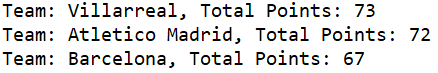
\includegraphics[width=8cm]{Images/function3.png}
    \caption{\small Function \texttt{get\_top\_teams} output}
    \label{fig:function3}
\end{figure}
@*)
\end{lstlisting}
\vspace{2em}
\subsection{Triggers}
\begin{lstlisting}[language=SQL, caption=\small Triggers (\texttt{DBTriggers.sql} file)]
-- Trigger for the Stadiums table to enforce a minimum capacity
CREATE OR REPLACE TRIGGER check_if_stadium_capacity_is_big_enough BEFORE
    INSERT OR UPDATE ON stadiums
    FOR EACH ROW
DECLARE
    capacity_too_small EXCEPTION;
BEGIN
    IF :new.capacity < 1000 THEN
        RAISE capacity_too_small;
    END IF;
EXCEPTION
    WHEN capacity_too_small THEN
        raise_application_error(-20001, 'Stadium capacity must be at least 1000.');
END;

-- Example to check the trigger
-- INSERT INTO stadiums VALUES (1111,'El Sadar','Pamplona',100);
-- Trigger for the Matches table to validate scores
CREATE OR REPLACE TRIGGER check_if_match_score_is_correct BEFORE
    INSERT OR UPDATE ON matches
    FOR EACH ROW
BEGIN
    IF :new.home_team_score < 0 OR :new.away_team_score < 0 THEN
        raise_application_error(-20002, 'Invalid match scores.');
    END IF;
END;

-- Example to check the trigger
-- INSERT INTO matches VALUES (1111, TO_DATE('2023-08-05', 'YYYY-MM-DD'), -3, 2, 'Antonio Mateu Lahoz', 1, 1, 2, 1);


-- Trigger for the Matches table to validate match date
CREATE OR REPLACE TRIGGER check_if_match_date_is_valid BEFORE
    INSERT OR UPDATE ON matches
    FOR EACH ROW
BEGIN
    IF :new.match_date < sysdate THEN
        raise_application_error(-20003, 'Match date cannot be in the past.');
    END IF;
END;

-- Example to check the trigger
-- INSERT INTO matches VALUES (11111, TO_DATE('2021-08-05', 'YYYY-MM-DD'), 3, 2, 'Antonio Mateu Lahoz', 1, 1, 2, 1);


-- Trigger for the Matches table to validate match week
CREATE OR REPLACE TRIGGER check_if_match_week_is_valid BEFORE
    INSERT OR UPDATE ON matches
    FOR EACH ROW
BEGIN
    IF :new.match_week < 1 OR :new.match_week > 48 THEN
        raise_application_error(-20004, 'Match week must be between 1 and 38.');
    END IF;
END;

-- Example to check the trigger
-- INSERT INTO matches VALUES (23228, TO_DATE('2025-03-29', 'YYYY-MM-DD'), 1, 1, 'Aliyar Aghayev', 410, 5, 2, 5);


-- Trigger for the Matches table to validate home and away teams
CREATE OR REPLACE TRIGGER check_if_home_and_away_teams_are_different BEFORE
    INSERT OR UPDATE ON matches
    FOR EACH ROW
BEGIN
    IF :new.home_team_id = :new.away_team_id THEN
        raise_application_error(-20005, 'Home and away teams must be different.');
    END IF;
END;

-- Example to check the trigger
-- INSERT INTO matches VALUES (238, TO_DATE('2025-03-29', 'YYYY-MM-DD'), 1, 1, 'Aliyar Aghayev', 40, 2, 2, 5);


-- Trigger for Teams table to enforce a constraint on the manager's name length
CREATE OR REPLACE TRIGGER check_manager_name_length
BEFORE INSERT OR UPDATE ON teams
FOR EACH ROW
BEGIN
    IF LENGTH(:new.manager_name) > 80 THEN
        RAISE_APPLICATION_ERROR(-20001, 'Manager name cannot exceed 80 characters.');
    END IF;
END;

-- Example to check the trigger
-- INSERT INTO teams VALUES (2132,'Barcelona',TO_DATE('1899-11-29', 'YYYY-MM-DD'),1,'Xavierdddddddddsdfsdfsdddddddddddddddddddddddddddddddddddddd
-- ddddddddddddddddddddddddddddddd Hernandez Creus');
\end{lstlisting}
\vspace{2em}
\subsection{Package}
\begin{lstlisting}[language=SQL, caption=\small Package (\texttt{DBPackage.sql} file), escapeinside={(*@}{@*)}]
-- Package containing procedure for updating the capacity of specific stadium and procedure for generation of report with match scores
CREATE OR REPLACE PACKAGE football_package IS
    PROCEDURE update_stadium_capacity (
        stadium_id   IN NUMBER,
        new_capacity IN NUMBER
    );

    PROCEDURE generate_match_scores_report (
        match_week IN NUMBER
    );

END football_package;
/
(*@\clearpage@*)
CREATE OR REPLACE PACKAGE BODY football_package IS

    PROCEDURE update_stadium_capacity (
        stadium_id   IN NUMBER,
        new_capacity IN NUMBER
    ) IS
    BEGIN
        UPDATE stadiums
        SET capacity = new_capacity
        WHERE id = stadium_id;

    END update_stadium_capacity;


    PROCEDURE generate_match_scores_report (
        match_week IN NUMBER
    ) IS
        CURSOR match_scores_cursor IS
        SELECT m.id,
               m.match_date,
               m.home_team_score,
               m.away_team_score,
               ht.name AS home_team_name,
               at.name AS away_team_name
        FROM matches m
            INNER JOIN teams ht ON m.home_team_id = ht.id
            INNER JOIN teams at ON m.away_team_id = at.id
        WHERE m.match_week = match_week;

    BEGIN
        FOR match_score IN match_scores_cursor LOOP
            dbms_output.put_line('Match ID: ' || match_score.id);
            dbms_output.put_line('Match Date: ' || match_score.match_date);
            dbms_output.put_line('Home Team: ' || match_score.home_team_name);
            dbms_output.put_line('Home Team Score: ' || match_score.home_team_score);
            dbms_output.put_line('Away Team: ' || match_score.away_team_name);
            dbms_output.put_line('Away Team Score: ' || match_score.away_team_score);
            dbms_output.put_line('------------------------');
        END LOOP;
    END generate_match_scores_report;

END football_package;

-- Example of update_stadium_capacity usage from the football_package
-- BEGIN
--     football_package.update_stadium_capacity(1, 20000);
-- END;

-- Example of generate_match_scores_report usage from the football_package
-- BEGIN
--     football_package.generate_match_scores_report(12);
-- END;
(*@
\begin{figure}[htp]
    \centering
    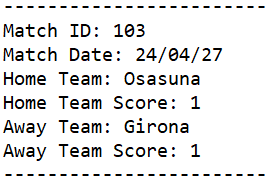
\includegraphics[width=5cm]{Images/packageReport.png}
    \caption{\small Procedure \texttt{generate\_match\_scores\_report} output}
    \label{fig:packageReport}
\end{figure}
@*)
\end{lstlisting}
\clearpage
\subsection{Other additional database structures}
\begin{lstlisting}[language=SQL, caption=\small Other additional structures (\texttt{DBAdditionalStructures.sql} file), escapeinside={(*@}{@*)}]
-- Simple view to show members' stats
CREATE VIEW member_stats_view AS
    SELECT m.id,
           m.name,
           m.surname,
           m.dob,
           m.salary,
           m.nationality,
           t.name                           AS team_name,
           COUNT(DISTINCT ma.id)            AS matches_played,
           COUNT(DISTINCT ma.id) * m.salary AS total_earnings,
           SUM(CASE
                    WHEN ma.home_team_id = m.team_id THEN
                        ma.home_team_score
                    ELSE
                        ma.away_team_score
               END) AS goals_scored
    FROM members m
        JOIN teams t ON m.team_id = t.id
        LEFT JOIN matches ma ON m.team_id = ma.home_team_id
                                OR m.team_id = ma.away_team_id
    GROUP BY m.id,
             m.name,
             m.surname,
             m.dob,
             m.salary,
             m.nationality,
             t.name;

-- Example of member_stats_view usage
-- SELECT * FROM member_stats_view;
(*@
\begin{figure}[htp]
    \centering
    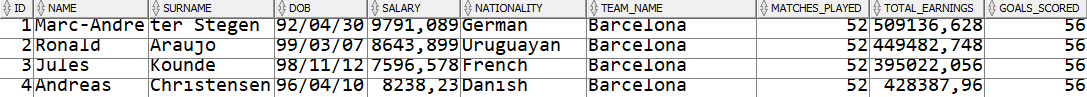
\includegraphics[width=15cm]{Images/view.png}
    \caption{\small View \texttt{member\_stats\_view} output}
    \label{fig:view}
\end{figure}
@*)

-- XML report
DECLARE
    xml_data XMLTYPE;
BEGIN
    xml_data := xmltype('<stadiums>
                        <stadium>
                          <id>11</id>
                          <name>ttt</name>
                          <city>test</city>
                          <capacity>12374</capacity>
                        </stadium>
                        <stadium>
                          <id>12</id>
                          <name>Sds</name>
                          <city>Ssdf</city>
                          <capacity>32774</capacity>
                        </stadium>
                      </stadiums>');

    FOR s IN (
        SELECT
            extractvalue(value(st),
                         '/stadium/id')       AS id,
            extractvalue(value(st),
                         '/stadium/name')     AS name,
            extractvalue(value(st),
                         '/stadium/city')     AS city,
            extractvalue(value(st),
                         '/stadium/capacity') AS capacity
        FROM
          TABLE ( xmlsequence(xml_data.extract('/stadiums/stadium')) ) st
    ) LOOP
        INSERT INTO stadiums (id,
                              name,
                              city,
                              capacity
        ) VALUES (s.id,
                  s.name,
                  s.city,
                  s.capacity);
    END LOOP;

    COMMIT;
END;

-- SELECT * FROM stadiums;


-- Pipelined function
CREATE OR REPLACE TYPE ticket_profit_type AS OBJECT (
    match_id NUMBER,
    profit   NUMBER
);
/

CREATE OR REPLACE TYPE ticket_profit_table_type AS
    TABLE OF ticket_profit_type;
/
(*@\clearpage@*)
CREATE OR REPLACE FUNCTION calculate_ticket_profit RETURN ticket_profit_table_type
    PIPELINED
AS
    v_profit NUMBER;
BEGIN
    FOR rec IN (SELECT t.match_id,
                       ( t.price * t.quantity ) AS profit
                FROM tickets t
    ) LOOP
        v_profit := rec.profit;
        PIPE ROW ( ticket_profit_type(rec.match_id, v_profit) );
    END LOOP;

    RETURN;
END;

SELECT match_id,
       profit
FROM 
  TABLE ( calculate_ticket_profit );
(*@
\begin{figure}[htp]
    \centering
    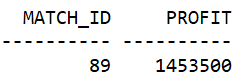
\includegraphics[width=4cm]{Images/pipe.png}
    \caption{\small Pipelined function \texttt{calculate\_ticket\_profit} output}
    \label{fig:pipe}
\end{figure}
@*)
\end{lstlisting}

\end{document}
